% \VignetteIndexEntry{R4RNA}
% \VignetteDepends{R4RNA}
% \VignetteKeywords{RNA secondary structure arc diagram visualization}
% \VignettePackage{R4RNA}

\documentclass[letterpaper]{article}
\usepackage{graphicx}
\usepackage{wrapfig}
\usepackage{fullpage}
\usepackage{hyperref}
\usepackage{caption}

\title{wisard: A package to perform the weighted interval scheduling algorithm}
\author{Robert Buecking}
\date{\today}

\usepackage{Sweave}
\begin{document}
\Sconcordance{concordance:wisard.tex:wisard.Rnw:%
1 16 1 1 0 35 1 1 2 1 0 1 2 1 0 1 1 5 0 1 2 15 0 1 2 74 0 1 2 356 1}


\setkeys{Gin}{width=\textwidth}

\maketitle
\tableofcontents

\section{Installation}

requires devtools package
\begin{Schunk}
\begin{Sinput}
	> library(devtools)
	> setwd(wisard/..)
	> install("wisard")
\end{Sinput}
\end{Schunk}

\section{wisard}

\subsection{Algorithm}

The wisard package contains functions to perform the wighted interval scheduling
algorithm on a set of intervals. Primarily, this package is intended to remove
overlapping alignments from whole genome alignments created with BLAST, but it
can be applied to any other form of weighted intervals to find the highest
scoring set of non-overlapping intervals. The weighted interval scheduling
algorithm is a dynamic programming algorithm that finds the highest scoring
path of compatible intervals through a set of weighted intervals as depicted
in figure \ref{fig:algo}. The functions are easiy to modify with regard to
overlap criteria and weighting scheme.

\begin{figure}[h]
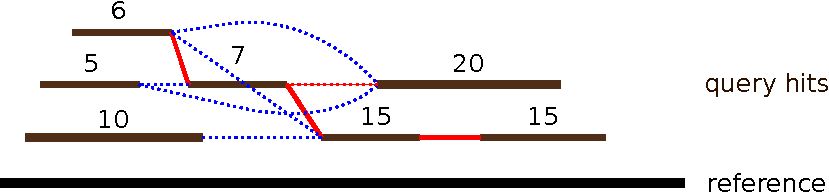
\includegraphics{algorithm.pdf}
\caption{Highest scoring path of compatible intervals}
\label{fig:algo}
\end{figure}

The package additionally contains a function to parse BLAST xml-output with a
single subject and query sequence.

The workflow is demonstrated in a short example below. Input can be a BLAST-result as XML, as explained below or any other format transformed into a GRanges object.

\subsection{Reading a BLAST xml-output file}

The function read\_blast\_xml can be used to parse a BLAST xml-output file
generated by NCBI-BLAST using -outfmt 5 or AB-BLAST using -mformat=7.

\begin{Schunk}
\begin{Sinput}
> library(wisard)
> # Reading a BLAST xml-file
> xml_file <- system.file("extdata", "example.xml", package = 'wisard')
> blast_result <- read_blast_xml(xml_file, grange_output = T, keep_sequences = F)
\end{Sinput}
\begin{Soutput}
[1] "file is from blastn"
\end{Soutput}
\begin{Sinput}
> # Metadata contained in xml-file
> blast_result$metadata
\end{Sinput}
\begin{Soutput}
  Statistics_db.num Statistics_db.len Statistics_hsp.len Statistics_eff.space
1                 1          10327335                 68          5.60758e+13
  Statistics_kappa Statistics_lambda Statistics_entropy program
1            0.104             0.988                0.4  blastn
                                                             query_name
1 Lactobacillus zhachilii strain HBUAS52074 chromosome, complete genome
       query_ID query_len Parameters_expect Parameters_sc.match
1 NZ_CP031933.2   2714973                10                   1
  Parameters_sc.mismatch Parameters_gap.open Parameters_gap.extend
1                     -1                   1                     2
\end{Soutput}
\begin{Sinput}
> # Alignments contained in the xml file
> blast_result$alignments
\end{Sinput}
\begin{Soutput}
GRanges object with 549 ranges and 20 metadata columns:
           seqnames          ranges strand |   Hsp_num Hsp_bit.score Hsp_score
              <Rle>       <IRanges>  <Rle> | <numeric>     <numeric> <numeric>
    1 NZ_CP011125.1 8624113-8625463      + |         1       1085.13       759
    2 NZ_CP011125.1 8618246-8619596      + |         2       1085.13       759
    3 NZ_CP011125.1 8620573-8621704      + |         3       921.212       644
    4 NZ_CP011125.1 8614706-8615837      + |         4       921.212       644
    5 NZ_CP011125.1 8621992-8622990      + |         5       537.784       375
  ...           ...             ...    ... .       ...           ...       ...
  545 NZ_CP011125.1 5009294-5009466      - |       545       43.1761        28
  546 NZ_CP011125.1 5009285-5009457      - |       546       43.1761        28
  547 NZ_CP011125.1 6349092-6349267      - |       547       43.1761        28
  548 NZ_CP011125.1 9910129-9910337      - |       548       43.1761        28
  549 NZ_CP011125.1 4320937-4321200      - |       549       43.1761        28
        Hsp_evalue Hsp_query.from Hsp_query.to Hsp_hit.from.1 Hsp_query.frame
         <numeric>      <numeric>    <numeric>      <numeric>       <numeric>
    1            0        1993721      1995068        8624113               1
    2            0        1993721      1995068        8618246               1
    3 2.72951e-264        1990664      1991793        8620573               1
    4 2.72951e-264        1990664      1991793        8614706               1
    5  7.2365e-149        1992046      1993036        8621992               1
  ...          ...            ...          ...            ...             ...
  545      5.64262         527497       527669        5009294               1
  546      5.64262         527425       527597        5009285               1
  547      5.64262        2096151      2096326        6349092               1
  548      5.64262         431628       431836        9910129               1
  549      5.64262        2039609      2039869        4320937               1
      Hsp_hit.frame Hsp_identity Hsp_positive  Hsp_gaps Hsp_align.len   seq_len
          <numeric>    <numeric>    <numeric> <numeric>     <numeric> <numeric>
    1             1         1063         1063         7          1353  10327335
    2             1         1063         1063         7          1353  10327335
    3             1          892          892         4          1133  10327335
    4             1          892          892         4          1133  10327335
    5             1          716          716        28          1009  10327335
  ...           ...          ...          ...       ...           ...       ...
  545            -1          103          103         2           174  10327335
  546            -1          103          103         2           174  10327335
  547            -1          102          102      <NA>           176  10327335
  548            -1          121          121         2           210  10327335
  549            -1          151          151         5           265  10327335
      query_len      query_id raw_score        ID filter_pass
      <numeric>   <character> <numeric> <integer>   <logical>
    1   2714973 NZ_CP031933.2       759         1        TRUE
    2   2714973 NZ_CP031933.2       759         2        TRUE
    3   2714973 NZ_CP031933.2       644         3        TRUE
    4   2714973 NZ_CP031933.2       644         4        TRUE
    5   2714973 NZ_CP031933.2       375         5        TRUE
  ...       ...           ...       ...       ...         ...
  545   2714973 NZ_CP031933.2        28       545        TRUE
  546   2714973 NZ_CP031933.2        28       546        TRUE
  547   2714973 NZ_CP031933.2        28       547        TRUE
  548   2714973 NZ_CP031933.2        28       548        TRUE
  549   2714973 NZ_CP031933.2        28       549        TRUE
                       query_ranges
                          <GRanges>
    1 NZ_CP031933.2:1993721-1995068
    2 NZ_CP031933.2:1993721-1995068
    3 NZ_CP031933.2:1990664-1991793
    4 NZ_CP031933.2:1990664-1991793
    5 NZ_CP031933.2:1992046-1993036
  ...                           ...
  545   NZ_CP031933.2:527497-527669
  546   NZ_CP031933.2:527425-527597
  547 NZ_CP031933.2:2096151-2096326
  548   NZ_CP031933.2:431628-431836
  549 NZ_CP031933.2:2039609-2039869
  -------
  seqinfo: 1 sequence from an unspecified genome
\end{Soutput}
\end{Schunk}

\subsection{Caclulating the BLAST sum score}
\begin{Schunk}
	\begin{Sinput}
		> # calculating the BLAST sum score of a set of alignments:
		> sum_score(blast_result$alignments$raw_score, blast_result$metadata)
	\end{Sinput}
	\begin{Soutput}
		[1] 25028.66
	\end{Soutput}
\end{Schunk}

\subsection{Filter BLAST results}

The function filter\_blast can be used to filter the blast results
\begin{Schunk}
	\begin{Sinput}
		> # filter records:
		> blast_result$alignments <- filter_blast(blast_result$alignments,
		+                                         min_len = 10,
		+                                         max_e = 1,
		+                                         min_identity = 0)
	\end{Sinput}
	\begin{Soutput}
		[1] "Number of alignments filtered out"
		[1] 92
		[1] "Number of alignments that passed filter"
		[1] 457
	\end{Soutput}
\end{Schunk}


\subsection{Run the WIS algorithm}
The function run\_get\_wis runs the WIS algorithm

\begin{Schunk}
	\begin{Sinput}
		> # run wis
		> wis_results <- run_get_wis(blast_result$alignments, is_circular = T,
		+                            use_strand = T,
		+                            score_col = "raw_score")
	\end{Sinput}
	\begin{Soutput}
		[1] "strand yes, frame no"
		[1] "analyzing + strand"
		calculate wis for start alignment  1 
		max score is:  11617 
		[1] "analyzing - strand"
		calculate wis for start alignment  1 
		max score is:  10515 
	\end{Soutput}
\end{Schunk}



\subsection{Run the greedy algorithm}
The function greedy\_algorithm runs the WIS algorithm

\begin{Schunk}
	\begin{Sinput}
		> # run greedy
		> greedy_results <- greedy_algorithm(blast_result$alignments,
		+                                    max_score = "raw_score",
		+                                    is_circular = T,
		+                                    use_strand = T)
	\end{Sinput}
	\begin{Soutput}
		[1] "in greedy"
	\end{Soutput}
	\begin{Sinput}
		> length(blast_result$alignments)
	\end{Sinput}
	\begin{Soutput}
		[1] 457
	\end{Soutput}
	\begin{Sinput}
		> length(greedy_results)
	\end{Sinput}
	\begin{Soutput}
		[1] 291
	\end{Soutput} 
\end{Schunk}
%
% transat_file <- system.file("extdata", "helix.txt", package = "R4RNA")
% transat <- readHelix(transat_file)
%
% message("RFAM structure in dot bracket format")
% known_file <- system.file("extdata", "vienna.txt", package = "R4RNA")
% known <- readVienna(known_file)
%
% message("Work with basepairs instead of helices for more flexibility")
% message("Breaks all helices into helices of length 1")
% transat <- expandHelix(transat)
% known <- expandHelix(known)
% @
%
% For multiple entities you can use just updated ``helix'' format. Below, we read predicted and known structures.
%
% <<>>=
% #read fasta
% fasta_file.mltp <- system.file("extdata", "fasta.mltp.txt", package = "R4RNA")
% fasta.mltp <- readBStringSet(fasta_file.mltp)
% #read helix
% transat.file.mltp <- system.file("extdata", "transat.helix.mltp.txt" ,package = "R4RNA")
% helix.transat.mltp <- readHelixMltp(transat.file.mltp)
% known.file.mltp <- system.file("extdata", "known.helix.mltp.txt", package = "R4RNA")
% helix.known.mltp <- readHelixMltp(known.file.mltp)
%
% is.helix.mltp(helix.transat.mltp)
% helix.transat.exp <- expandHelixMltp(helix.transat.mltp)
% helix.known.exp <- expandHelixMltp(helix.known.mltp)
%
% is.helix.mltp(helix.transat.exp)
% is.helix.mltp(helix.known.exp)
% @
%
%
% \subsection{Basic Arc Diagram}
%
% The standard arc diagram, where the nucleotide sequence is the horizontal
% line running left to right from 5' to 3' at the bottom of the diagram.  Any
% two bases that base-pair in a secondary structure are connect with an arc.
%
% <<fig=TRUE,eps=FALSE,height=1.9>>=
% plotHelix(known, line = TRUE, arrow = TRUE)
% mtext("Known Structure", side = 3, line = -2, adj = 0)
% @
%
% Plot for multiple entities. Trans interactions are given by length equal 1.
% There is Single line and Double Line Modes.
% Single line:
%
% <<fig=TRUE,eps=FALSE,height=1.9>>=
% plotHelixMltpSingleLine(copy(helix.known.exp),scale = FALSE)
% mtext("Known Structure", side = 3, line = -2, adj = 0)
% @
%
% Double line:
% <<fig=TRUE,eps=FALSE,height=4,width=8>>=
% plotHelixMltpDoubleLine(copy(helix.known.exp),scale = FALSE)
% mtext("Known Structure", side = 3, line = -10, adj = 0)
% @
%
%
% \subsection{Multiple Structures}
%
% Two structures for the same sequence can be visualized simultaneously, allowing
% one to compare and contrast the two structures.
%
% <<fig=TRUE,eps=FALSE,height=4>>=
% plotDoubleHelix(transat, known, line = TRUE, arrow = TRUE)
% mtext("TRANSAT\nPredicted\nStructure", side = 3, line = -5, adj = 0)
% mtext("Known Structure", side = 1, line = -2, adj = 0)
% @
%
% <<fig=TRUE,eps=FALSE,height=4>>=
% plotDoubleHelixMltpSingleLine(helix.known.exp,helix.transat.exp,scale = FALSE)
% mtext("Predicted\nStructure", side = 1, line = -5, adj = 0)
% mtext("Known Structure", side = 3, line = -2, adj = 0)
% @
%
% <<fig=TRUE,eps=TRUE,height=4,width=8>>=
% plotDoubleHelixMltpDoubleLine(helix.known.exp,helix.transat.exp,stable = TRUE,scale = FALSE)
% mtext("Predicted\nStructure", side = 3, line = -5, adj = 1)
% mtext("Known Structure", side = 3, line = -5, adj = 0)
% @
%
%
% \subsection{Filtering Helices}
% Base-pairs can be associated with a value, such as energy stability or
% statistical probability, and we can easily filter out basepairs according to
% such rules.
%
% <<>>=
% message("Filter out helices above a certain p-value")
% transat <- transat[which(transat$value <= 1e-3), ]
% @
%
% \subsection{Colouring Structures}
% We can also assign colour to the structure according to base-pairs values.
%
% <<fig=TRUE,eps=FALSE,height=4.3>>=
% message("Assign colour to basepairs according to p-value")
% transat$col <- col <- colourByValue(transat, log = TRUE)
%
% message("Coloured encoded in 'col' column of transat structure")
% plotDoubleHelix(transat, known, line = TRUE, arrow = TRUE)
%
% legend("topright", legend = attr(col, "legend"), fill = attr(col, "fill"),
%     inset = 0.05, bty = "n", border = NA, cex = 0.75, title = "TRANSAT P-values")
% @
%
% Same can be done to multiple entitites.
%
% <<fig=TRUE,eps=FALSE,height=4,width=8>>=
% helix.transat.exp <- helix.transat.exp[,1:6]
% helix.transat.exp$col <- col <- colourByValueMltp(helix.transat.exp, log = TRUE)
%
% message("Coloured encoded in 'col' column of transat structure")
% plotDoubleHelixMltpSingleLine(helix.known.exp,helix.transat.exp,scale = FALSE)
%
% legend("topright", legend = attr(col, "legend"), fill = attr(col, "fill"),
% 	inset = 0.05, bty = "n", border = NA, cex = 0.75, title = "TRANSAT P-values")
% @
%
% <<fig=TRUE,eps=FALSE,height=4,width=8>>=
% helix.transat.exp <- helix.transat.exp[,1:6]
% helix.transat.exp$col <- col <- colourByValueMltp(helix.transat.exp, log = TRUE)
%
% message("Coloured encoded in 'col' column of transat structure")
% plotDoubleHelixMltpDoubleLine(helix.known.exp,helix.transat.exp,scale = FALSE,stable = TRUE)
%
% legend("topright", legend = attr(col, "legend"), fill = attr(col, "fill"),
% 	inset = 0.05, bty = "n", border = NA, cex = 0.75, title = "TRANSAT P-values")
% @
%
%
% \subsection{Overlapping Multiple Structures}
%
% A neat way of visualizing the concordance between two structure is an
% overlapping structure diagram, which we can use to overlap the predicted TRANSAT
% structure and the known RFAM structure.  Predicted basepairs that exist in the
% known structure are drawn above the line, and those predicted that are not known
% to exist are drawn below.  Those known but unpredicted are shown in black above
% the line.
%
% <<fig=TRUE,eps=FALSE,height=4.4>>=
% plotOverlapHelix(transat, known, line = TRUE, arrow = TRUE, scale = FALSE)
% @
%
% Same can be done to multiple entitites.
%
% <<fig=TRUE,eps=FALSE,height=4>>=
% plotComparisonHelixMltpSingleLine(helix1 = helix.known.exp[,1:6],helix2 = helix.transat.exp[,1:6],scale = FALSE)
% mtext("Known Structure", side = 3, line = -5, adj = 0)
% mtext("Predicted\nStructure", side = 1, line = -2, adj = 0)
% @
%
% <<fig=TRUE,eps=FALSE,height=4>>=
% plotComparisonHelixMltpDoubleLine(helix1 = helix.known.exp[,1:6],helix2 = helix.transat.exp[,1:6],scale = FALSE)
% mtext("Known Structure", side = 3, line = -5, adj = 0)
% mtext("Predicted\nStructure", side = 1, line = -2, adj = 0)
% @
%
%
% \subsection{Visualizing Multiple Sequence Alignments}
%
% In addition to visualizing the structure alone, we can also visualize a
% secondary structure along with aligned nucleotide sequences.  In the following,
% we will read in a multiple sequence alignment obtained from RFAM, and visualize
% the known structure on top of it.
%
% We can also annotate the alignment colours according to their agreement with the
% known structure.  If a sequence can form as basepair as dictated by the structure,
% the basepair is coloured green, else red.  For green basepairs, if a mutation
% has occured, but basepairing potential is retained, it is coloured in blue
% (dark for mutations in both bases, light for single-sided mutation).  Unpaired
% bases are in black and gaps are in grey.
%
% <<fig=TRUE,eps=FALSE,height=2.4>>=
% message("Multiple sequence alignment of interest")
% library(Biostrings)
% fasta_file <- system.file("extdata", "fasta.txt", package = "R4RNA")
% fasta <- as.character(readBStringSet(fasta_file))
%
% message("Plot covariance in alignment")
% plotCovariance(fasta, known, cex = 0.5)
% @
%
% Same can be done to multiple entitites.
%
% <<fig=TRUE,eps=FALSE,height=4>>=
% message("Multiple sequence alignment of interest")
% fasta_file.mltp <- system.file("extdata", "fasta.mltp.txt", package = "R4RNA")
% fasta.mltp <- readBStringSet(fasta_file.mltp)
%
% message("Plot covariance in alignment")
% plotCovarianceMltpSingleLine(helix = helix.transat.exp[,1:7],msa = fasta.mltp,grid = FALSE,scale = FALSE)
% @
%
%
% <<fig=TRUE,eps=FALSE,height=4>>=
% message("Multiple sequence alignment of interest")
% fasta_file.mltp <- system.file("extdata", "fasta.mltp.txt", package = "R4RNA")
% fasta.mltp <- readBStringSet(fasta_file.mltp)
%
% message("Plot covariance in alignment")
% plotCovarianceMltpDoubleLine(helix = helix.transat.exp[,1:7],
%                              msa = fasta.mltp,grid = FALSE, legend = FALSE,scale = FALSE)
% @
%
%
%
% \subsection{Multiple Sequence Alignements with Annotated Arcs}
%
% Arcs can be coloured as usual.  It should be noted that structures with
% conflicting basepairs (arcs sharing a base) cannot be visualized properly
% on a multiple sequence alignment, and are typically filtered out (\textit{e.g.}
% drawn in grey here).
%
% <<fig=TRUE,eps=FALSE,height=2.7>>=
% plotCovariance(fasta, transat, cex = 0.5, conflict.col = "grey")
% @
%
% Same can be done to multiple entitites.
%
% <<fig=TRUE,eps=FALSE,height=4,width=8>>=
% message("Multiple sequence alignment of interest")
% fasta_file.mltp <- system.file("extdata", "fasta.mltp.txt", package = "R4RNA")
% fasta.mltp <- readBStringSet(fasta_file.mltp)
%
% message("Plot covariance in alignment")
% plotCovarianceMltpSingleLine(helix = helix.transat.exp[,1:7],msa = fasta.mltp,
%                              conflict.col = "grey",legend = TRUE,grid = FALSE,scale = FALSE)
% @
%
% <<fig=TRUE,eps=FALSE,height=4,width=8>>=
% message("Multiple sequence alignment of interest")
% fasta_file.mltp <- system.file("extdata", "fasta.mltp.txt", package = "R4RNA")
% fasta.mltp <- readBStringSet(fasta_file.mltp)
%
% message("Plot covariance in alignment")
% plotCovarianceMltpDoubleLine(helix = helix.transat.exp[,1:7],msa = fasta.mltp,
%                              conflict.col = "grey",grid = FALSE,scale = FALSE)
% @
%
%
% \subsection{Additional Colouring Methods}
%
% Various other methods of colour arcs exist, along with many options to control
% appearances:
%
% \subsubsection{Colour By Covariation (with alignment as blocks)}
%
% <<fig=TRUE,eps=FALSE,height=2.4>>=
% col <- colourByCovariation(known, fasta, get = TRUE)
% plotCovariance(fasta, col, grid = TRUE, legend = FALSE)
% legend("topright", legend = attr(col, "legend"), fill = attr(col, "fill"),
%     inset = 0.1, bty = "n", border = NA, cex = 0.37, title = "Covariation")
% @
%
% <<fig=TRUE,eps=FALSE,height=4,width=8>>=
%
% col <- colourByCovariationMltp(helix = helix.transat.exp,msa = fasta.mltp,get = TRUE)
%
% plotCovarianceMltpSingleLine(helix = col,msa = fasta.mltp,grid = TRUE,scale = FALSE)
% legend("topright", legend = attr(col, "legend"), fill = attr(col, "fill"),
%        inset = 0.1, bty = "n", border = NA, cex = 0.5, title = "Covariation")
% @
%
%
%
% \subsubsection{Colour By Conservation (with custom alignment colours)}
%
% <<fig=TRUE,eps=FALSE,height=2.2>>=
% custom_colours <- c("green", "blue", "cyan", "red", "black", "grey")
% plotCovariance(fasta, col <- colourByConservation(known, fasta, get = TRUE),
%     palette = custom_colours, cex = 0.5)
% legend("topright", legend = attr(col, "legend"), fill = attr(col, "fill"),
%     inset = 0.15, bty = "n", border = NA, cex = 0.75, title = "Conservation")
% @
%
% <<fig=TRUE,eps=FALSE,height=4,width=8>>=
% custom_colours <- c("green", "blue", "cyan", "red", "black", "grey")
% plotCovarianceMltpSingleLine(msa = fasta.mltp, helix = col <- colourByConservationMltp(helix = helix.transat.exp,msa = fasta.mltp,get = TRUE,cols = custom_colours),palette = custom_colours,scale = FALSE)
% legend("topright", legend = attr(col, "legend"), fill = attr(col, "fill"),
% 	inset = 0.15, bty = "n", border = NA, cex = 0.75, title = "Conservation")
% @
%
%
% \subsubsection{Colour By Percentage Canonical Basepairs (with custom arc colours)}
%
% <<fig=TRUE,eps=FALSE,height=2.2>>=
% col <- colourByCanonical(known, fasta, custom_colours, get = TRUE)
% plotCovariance(fasta, col, base.colour = TRUE, cex = 0.5)
% legend("topright", legend = attr(col, "legend"), fill = attr(col, "fill"),
%     inset = 0.15, bty = "n", border = NA, cex = 0.75, title = "% Canonical")
% @
%
% <<fig=TRUE,eps=FALSE,height=4,width=8>>=
% col <- colourByCanonicalMltp(helix = helix.transat.exp,msa = fasta.mltp,get = TRUE)
% plotCovarianceMltpSingleLine(helix = col,msa = fasta.mltp,scale = FALSE)
% legend("topright", legend = attr(col, "legend"), fill = attr(col, "fill"),
% 	inset = 0.15, bty = "n", border = NA, cex = 0.75, title = "% Canonical")
% @
%
%
% \subsubsection{Colour Pseudoknots (with CLUSTALX-style alignment)}
%
% <<fig=TRUE,eps=FALSE,height=2.2>>=
% col <- colourByUnknottedGroups(known, c("red", "blue"), get = TRUE)
% plotCovariance(fasta, col, base.colour = TRUE, legend = FALSE, species = 23, grid = TRUE, text = TRUE, text.cex = 0.2, cex = 0.5)
% @
%
% <<fig=TRUE,eps=FALSE,height=4,width=8>>=
% col <- colourByUnknottedGroupsMltp(helix = helix.transat.exp,cols = c("red","blue"),get = TRUE)
% plotCovarianceMltpSingleLine(helix = col,msa = fasta.mltp,base.colour = TRUE,scale = FALSE)
% @
%
% \subsection{Working with HiC data}
%
% HiC triangular format file obtained with straw
%
% <<>>=
% hic_file <- system.file("extdata", "GSE63525.chr10.chr11.500kb.txt", package = "R4RNA")
% helix_hic <- StrawToHelix(file = hic_file, chr1 = "chr10",chr2 = "chr11",scale = 500000)
% @
%
%
% Trimm low values of strength interactions. After update attribute for new generated helix file. And colour by value (interaction strength).
%
% <<>>=
% helix_hic.trimmed <- helix_hic[value > 40]
% attr(helix_hic.trimmed,"length") <- attr(helix_hic,"length")
% helix_hic.trimmed <- colourByValueMltp(helix_hic.trimmed,get = TRUE)
% @
%
% Plot figure from filtered data
%
% <<fig=TRUE,eps=FALSE,height=4,width=8>>=
% plotHelixMltpSingleLine(helix = helix_hic.trimmed,shape = "triangle",scale = FALSE)
% @
%
% Plot figure from filtered data in heatmap way
%
% <<fig=TRUE,eps=FALSE,height=4,width=8>>=
% plotHelixMltpSingleLine(helix = helix_hic.trimmed,shape = "heatmap",scale = FALSE)
% @
%
% \section{Session Information}
%
% The version number of R and packages loaded for generating the vignette were:
%
% <<echo=FALSE, results=tex>>=
% toLatex(sessionInfo())
%
% @

\end{document}
